\chapter[Results]{Results}
\label{Chap:Results}

\section{RXJ1720+2638}
\label{sec:rxj1720+2638}
RXJ1720+2638 (also known as RXJ1720.1+2638) is a cool core galaxy cluster at $z = 0.160$ \citep{Owers2011}. Early observations detected the presence of two cold fronts, an edge to the southeast and a plateau to the northwest \citep{Mazzotta2001}. This suggested the presence of a core dense cold gas cloud ($T \approx 4$ keV) embedded in the outer diffuse and hot ICM ($T\approx10$ keV), with the cold fronts likely arising via a minor merger. Weak gravitational lensing studies \citep{Okabe2010} and galaxy density mapping \citep{Owers2011} revealed the presence of a substructure $\sim550$ kpc north of the cluster core. \citet{Owers2011} suggest that a northward passage of this structure passing the core to the east, providing the perturbations to the core and inducing large scale gas sloshing. RXJ1720+2638 was one of the first two clusters where cold fronts and minihalos were found to have a spatial correlation, with minihalo emission bounded by the cold fronts of the ICM \citep{Mazotta2008}. 

A detailed spectral study was performed by \citet{Giacintucci2014a}, which analysed observations at six frequencies from 317 MHz to 8.4 GHz taken by the GMRT and VLA. To perform accurate comparison between these frequencies, the baselines range was limited to 1--50 k$\lambda$, to enforce a unified sampling of the uv plane. to This noted three primary sources of minihalo emission in the core region, the central radio galaxy (BCG, single power-law $\alpha = 0.87\pm0.03$), a head-tail radio galaxy to the northeast with the tail to the south ($\alpha = 1.05\pm0.04$, steepening down the tail), and the minihalo emission. The BCG was noted to be unresolved with no jets or lobes detected at scales $>1.4$ kpc. Higher angular resolution observations by the extended Multi-Element Radio Linked Interferometer Network (e-MERLIN) at 4.76 GHz found the BCG to exhibit sub-kpc jets \citep{Perrott2023}. The jets extend 0.8 kpc to the east and west, though uncertainty in the recovered flux may indicate further undetected extent. \citet{Giacintucci2014a} separate the emission into a 160 kpc central region and tail region extending 200 kpc to the south. These were found to have spectral indices of $\alpha_c = 1.0\pm0.1$ and $\alpha_t = 1.5\pm0.1$, respectively. The core region exhibits a relatively flat spectral index across the extent, while spectral steepening is observed along the tail. LOFAR images at 144 MHz support the flat spectral index in the core, with steepening across the cold fronts \citet{Savini2019}. The spectral index for the core is consistent to 4.86 GHz, however, the 8.44 GHz measurement was lower than predicted by the single power-law. Although this indicated possible steepening, the 4.86 GHz and 8.44 GHz observations had much poorer uv sampling, which may have caused flux losses from the filtering of large-scale emission. \citet{Perrott2021} perform a high-frequency measurement of the central region of the minihalo was made at 15.5 GHz, using the Arcminute Microkelvin Imager (AMI). They construct a model of the minihalo in the uv plane to account for the spatial filtering, finding the single power-law $\alpha = 1.0$ is consistent to 15.5 GHz.

\subsection{10 GHz observation}
In processing the observations for imaging, two contaminating sources were identified prior to minihalo flux estimation. This included the BCG within the minihalo emission and a variable AGN to the southwest. These were modelled individually per dataset with a uvcut of 15 k$\lambda$ and subtracted. The head-tail source was sufficiently cleaned and tail emission isolated from that of the minihalo. A balance of beam sensitivity and PSF suppression was obtained using a \texttt{robust} of 1. Scales were set to $[0, 4, 8, 16, 32]$ with a \texttt{smalscalebias} of $-0.5$. \citet{Giacintucci2014a} supply details of the masking region, including the separation of centre and tail regions. This allowed a reproduction of these regions for analysis and accurate comparison to previous studies.\stickynote{I also have a 1--50 klambda image} 

The total minihalo flux was measured as $8.72\pm0.44$ mJy, with the majority $7.76\pm0.39$ mJy attributed to the central region and only $0.96\pm0.08$ mJy from the tail. The measured flux densities for relevant sources and regions are provided in Table \ref{tab:rxj1720+2638_flux}. The 10 GHz image is shown in Figure \ref{fig:rxj1720+2638_image}. The spectral index is fit for the total flux, centre, tail, and BCG using values measured from \citet{Giacintucci2014a} (excluding 8.46 GHz) and shown in Figure \ref{fig:rxj1720+2638_seds}. The spectral index of the central minihalo region was $\alpha_c = 1.07\pm0.06$, with a steeper tail region of $1.26\pm0.06$. The central results agree well with the previous result, with the tail found to be slightly flatter on average.

The BCG was measured to vary $\sim\!$20\% over one year (between C and D-configuration runs) and $\sim\!$10\% over one month (subsequent D-configurations). This degree of variation may suggest a systematic calibration error between the D-configuration observations. A systematic offset of $0.7$\% was observed in the flux density models of the secondary calibrator for these observations, other point sources in the image were measured and no systematic offsets were observed. Because of this, and the presence active jets from the BCG, the variation is likely real. 

\begin{table}[h]
    \centering
    \begin{tabular}{l|ccccc}
        \toprule
        Source & Minihalo & Minihalo (Centre) & Minihalo (Tail) & BCG \\ 
        \midrule
        Flux (mJy) & $8.77\pm0.44$ & $7.76\pm0.39$ & $0.96\pm0.08$ & $1.27\pm0.2$\\
        \bottomrule
    \end{tabular}
    \caption{Flux density obtained for sources in RXJ1720+2638 at 10 GHz. The value for the BCG is given as the average of the observed fluxes, with error corresponding to the maximum and minimum obtained.}
    \label{tab:rxj1720+2638_flux}
\end{table}

\begin{figure}
    \centering
    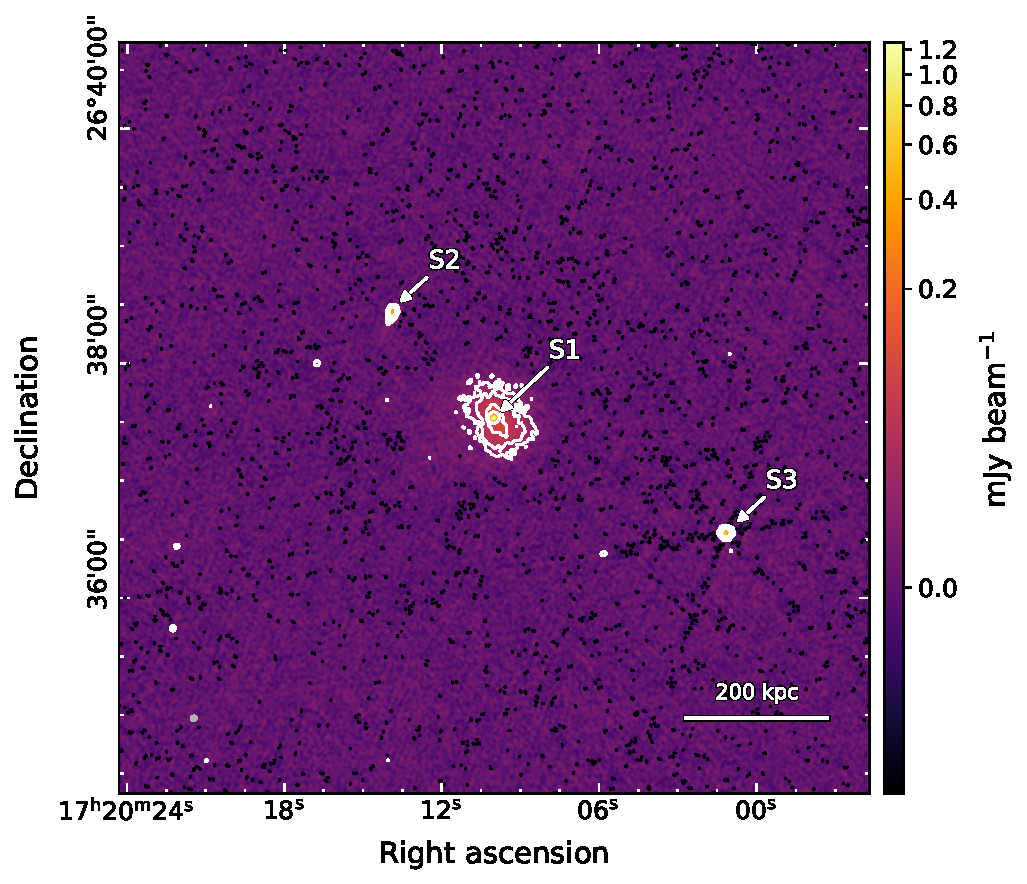
\includegraphics[width=0.85\textwidth]{Chapter5/vla_images/rxj1720.pdf}
    \caption{RXJ1720+2638. Point source subtracted 10 GHz observation with restoring beam $3.52"\times3.17"$ at position angle -34\textdegree{} and noise $1\sigma = 3.12$ $\mu$Jy beam$^{-1}$. Contour levels (white) are spaced in factors of two starting from 3$\sigma$. The masks used for flux estimation is shown in red, marking the centre (solid) and tail (dotted) regions. The green cross marks the location of the subtracted BCG.}
    \label{fig:rxj1720+2638_image}
\end{figure}

\begin{figure}
    \centering
    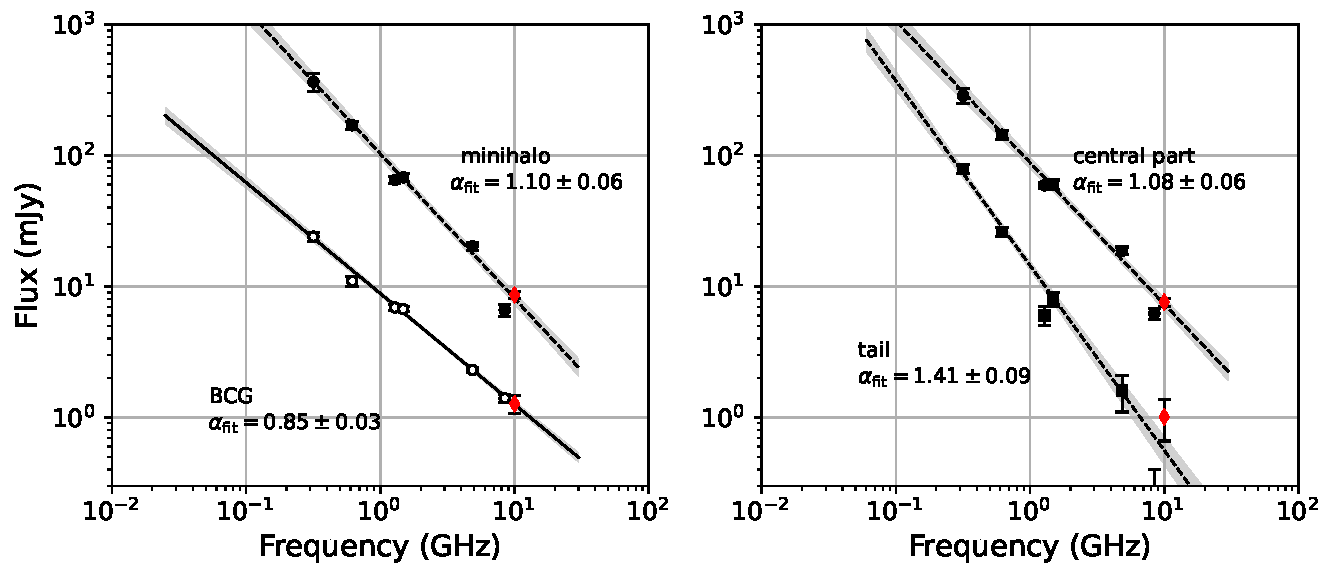
\includegraphics[width=\textwidth]{Chapter5/rxj1720_seds.pdf}
    \caption{RXJ1720+2368 radio spectra between 317 MHz and 10 GHz. \textit{Left Panel:} Spectrum of total minihalo (filled circles) and BCG (empty circles), red diamond denotes the 10 GHz measurement. The dotted line represents the minihalo power-law fit, solid line is BCG power-law spectrum, neither include the 8.44 GHz value. Grey shading as 1$\sigma$ error, slope and error are given in panel. \textit{Right Panel:} Spectrum of central (circles) and tail (squares) components. Dashed lines are are power-law fits over same range as left panel, grey shading indicates $1\sigma$ confidence, and slopes are reported.}
    \label{fig:rxj1720+2638_seds}
\end{figure}

\section{A478}

A478 is a nearby cool core cluster at a redshift of $z = 0.88$ \citep{Liu2024} . Chandra observations reveal a relaxed and highly elliptically symmetrical structure, with a central double-lobe BCG \citep{Sun2003, Bourdin2008}. The core temperature is $T \approx 1.54$ keV, increasing to $T\approx7.6$ keV at a radius of 260 kpc \citep{FanLam2024}. Two small ($\sim\!10$ kpc) X-ray cavities to the northeast and southwest are spatially aligned with the lobes of the BCG, indicating interaction between the BCG and ICM \citep{Sun2003}. A cold front is located 60 kpc to the southwest of the cluster \citep{Markevitch2003}. 

In the initial detection of minihalo emission, \citet{Giacintucci2014} note four several nearby radio sources to the minihalo. At 1.4 GHz, this includes the central BCG (S1), a head-tail to the east with a tail to the northwest (S4), a second head-tail within the tail of S4 with a tail to the northeast, and an unresolved source (S3) to the north of S2 and S4. The last source, S3, is likely to be a background source due to lacking optical correlations. \citet{Giacintucci2014} find the minihalo to be slightly extended more to the northeast ($R_{max} \sim 150$), compared to the other directions ($R_{min}\sim150$ kpc). This blends with the tail of S4, resulting in a large uncertainity in the flux estimate, due to difficulty in separating the tail and minihalo emission. They find the minihalo emission to be roughly constrained to the southwest cold front and a total flux $16.6\pm3$ mJy. LOFAR imaging at 144 MHz does not detect the diffuse minihalo emission, putting an upper bound on the spectral index of $\alpha < 1$ \citep{Savini2019}. Using archival GMRT data, \citet{Savini2019} finds S1 and S4 to have a spectral indices of $\sim\!1.1$ and $\sim\!0.6$, respectively, between 144 and 610 MHz. 

\subsection{10 GHz observation}
The observed minihalo region was much smaller than observed at 1.4 GHz, as to be expected. This resulted in only two contaminating sources, S1 and S4. The head-tail AGN doubled in brightness in the month between the D-configuration observations, causing severe PSF artefacts in the joint image. As such, this source was modelled on a per-dataset basis for the final self-calibration rounds. This variation was not observed in other point sources and could be attributed to a flare. The BCG exhibited time-variability within calibration error over all observations. The sources S2 and S3 are detected, but outside the radius of the observed minihalo. Three faint compact sources are located between S2 and the minihalo, but were spatially separate from the minihalo emission at the $3\sigma$ level. Point subtraction was then limited to S1 and S4 (including the tail) and used the standard 15 k$\lambda$ uv cut. The uv cut resulted in some emission remaining from S4, but as it was spatially distinct and the artefacts were successfully suppressed, this was left. The minihalo was modelled with scales $[0, 2, 4, 8, 16]$, \texttt{smallscalebias} of -0.5, and a \texttt{robust} of 1. The masking region was not clearly defined in \citep{Giacintucci2014}, so the mask used for flux estimation was determined by the $3\sigma$ region. 

The total minihalo flux was measured as $0.31 \pm 0.02$ mJy. The flux density of the BCG is $5.41 \pm 0.13$ mJy.

\begin{figure}
    \centering
    \includegraphics[width=0.85\textwidth]{Chapter5/vla_images/A478.pdf}
    \caption{RXJ1720+2638. Point source subtracted 10 GHz observation with restoring beam $5.55"\times4.96"$ at position angle -9.7\textdegree{} and noise $1\sigma = 1.88$ $\mu$Jy beam$^{-1}$. Contour levels (white) are spaced in factors of two starting from 3$\sigma$. The mask used for flux estimation is shown in by the dotted red line. The green cross marks the location of the subtracted BCG.}
    \label{fig:a478_image}
\end{figure}

\section{End}
Stick one big table of sources here? Ala Table 4 of G14 or Table 9 G19.